%-------------------------------------------------------------------------------
%                                PREAMBLE
%-------------------------------------------------------------------------------
\documentclass[usenames,dvipsnames,svgnames,10pt,aspectratio=169]{beamer}
\usefonttheme{professionalfonts}

% This theme uses TIKZ: compile twice with PDFLaTeX or LuaLaTeX.
%
%  Options:
%  - [clean]:    clean slides, i.e. logos and footbar are removed
%  - [kth]:      footbar style inspierd to the official KTH template
%  - [nicewave]: a different style of wave is used (not approved by FLOW)
%
\usetheme{flow}

\usepackage{hyperref,graphicx,lmodern}
\usepackage[utf8]{inputenc}
\usepackage{media9}
\usepackage{xcolor}
\usepackage{stmaryrd}
\usepackage{nicefrac}
\usepackage{multimedia}
\usepackage{multicol}
\usepackage{upgreek}
\usepackage[]{bm}
\usepackage[]{url}

\DeclareMathOperator{\sinc}{sinc}
\DeclareMathAlphabet{\mathcal}{OMS}{cmsy}{m}{n}
\DeclareMathAlphabet\mathbfcal{OMS}{cmsy}{b}{n}

\graphicspath{{imgs/}}
\setbeamertemplate{blocks}[rounded][shadow=true]

\DeclareMathOperator{\trace}{tr}

%-------------------------------------------------------------------------------
%                                TITLE PAGE
%-------------------------------------------------------------------------------
\title[Nonlinear Physics] % Short title used in footline
{
	Nonlinear physics, dynamical \\ systems and chaos theory
}

\author[J.-Ch.~Loiseau] % Presenting author in short form used in footline
{
	Jean-Christophe Loiseau
}
% - Give the names in the same order as the appear in the paper.
% - Underline the presenting author.

\institute[unused]
{
	\url{jean-christophe.loiseau@ensam.eu} \\
	DynFluid, \\
	Arts et M\'etiers ParisTech, France
}
% Keep it simple, no one is interested in your street address.

% University logo(s)
\logot{
\includegraphics[width=.128\paperwidth]{DynFluid_logo}}  % Top logo
\logob{
\includegraphics[width=0.128\paperwidth]{ENSAM_logo}} % Bottom logo
% \logoc[{
\includegraphics[width=.128\paperwidth]{limsi}}]{
\includegraphics[width=.128\paperwidth]{limsi}} % Corner logo
%
% Cover image: \cvrimg{x position}{y position}{cover image}
\cvrimg{.77}{.8}{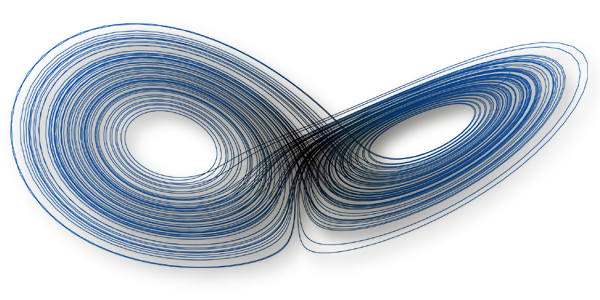
\includegraphics[width=.4\paperwidth]{cover.png}}

\date[unused]{ENSAM, Master 2, 2017--2018}

\begin{document}

\titleframe % Print the title as the first slide

%-------------------------------------------------------------------------------
%                           PRESENTATION SLIDES
%-------------------------------------------------------------------------------

\begin{frame}[t, c]{Today's menu}{Subharmonic cascade}
	\begin{itemize}
		\item So far, we have seen at least two sequences of bifurcations that cause a system to exhibit chaotic dynamics.
		\begin{itemize}
			\item[$\hookrightarrow$] \alert{\textbf{Logistic map}}: Sequence of period doubling bifurcations.
			\item[$\hookrightarrow$] \alert{\textbf{Lorenz system}}: For $0 \leq \rho \leq 25$, a supercritical pitchfork and a subcritical Hopf bifurcations occur before the creation of a stange attractor.
		\end{itemize}

		\bigskip

		\item These are two different routes to chaos. They are not the only ones though...

		\bigskip

		\item Today, we will focus exclusively on the sequence of period-doubling bifurcations
	\end{itemize}

	\vspace{1cm}
\end{frame}

\begin{frame}[t, c]{}
	\centering
	\vspace{1cm}

	{\Large \textbf{Logistic map}}

	\bigskip

	{\textgre{\textbf{A simple discrete-time model of population dynamics}}}

\end{frame}

\begin{frame}[t, c]{Logistic map}{A simple example}
	\begin{itemize}
		\item Let us consider once again the logistic map given by
		$$x_{k+1} = \mu x_k ( 1 - x_k),$$
		where $\mu$ is our control parameters.

		\bigskip

		\item We have studied this discrete-time system during Lecture 5.
	\end{itemize}

	\vspace{1cm}
\end{frame}

\end{document}
